\documentclass{article}
\usepackage[margin=1in]{geometry}
%math, symbols, drawing, plots, derivatives, table of contents editing, vectors, units
\usepackage{amsmath, amssymb, tikz, pgfplots, commath, tocloft, esvect, siunitx}
\usetikzlibrary{positioning, arrows}

\title{\vspace{-3ex}Advanced Function Notes}
\author{Jeffrey Gao\and More Contributors Later}
\renewcommand\thesubsubsection{\thesubsection{} \Alph{subsubsection}}
\renewcommand\labelitemi{--}
\cftpagenumbersoff{subsubsection}

\newcommand{\tsection}[1]{
	\section*{#1}
	\addcontentsline{toc}{section}{\protect\large #1}
}
\newcommand{\tsubsection}[1]{
	\subsection*{#1}
	\addcontentsline{toc}{subsection}{\protect\large #1}
}
\newcommand{\mv}[1]{
	\lVert\vv{#1}\rVert
}

\makeatletter
\g@addto@macro\bfseries{\boldmath}
\makeatother

\begin{document}
	\maketitle
	\tableofcontents
	\newpage
	\setcounter{section}{1}
	\tsection{Unit 1: Function Characteristics}
	\subsection{Functions}
	\subsubsection{Relations}
	A (binary) relation is defined as a set of ordered pairs $(x, y)$. A relation can be described using:
	\begin{itemize}
		\item words
		\item graphs
		\item equations
		\item inequalities
		\item lists of ordered pairs
		\item mapping diagrams
	\end{itemize}
	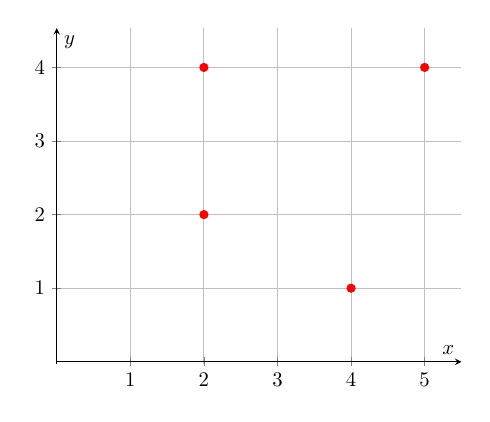
\begin{tikzpicture}[scale=.75]
		\begin{axis}[
			scatter/classes={a={draw=red,fill=red}},
			axis y line*=left,
			axis x line*=bottom,
			grid=both,
			ymin=0,
			xmin=0,
			ymax=4.5,
			xmax=5.5,
			axis equal,
			axis lines=middle,
			xlabel=$x$,
			ylabel=$y$,
			xtick distance=1,
			ytick distance=1
		]
		\addplot[scatter,only marks,scatter src=explicit symbolic]
		table[meta=label] {
			x y label
			2 2 a
			2 4 a
			4 1 a
			5 4 a
		};
		\end{axis}
	\end{tikzpicture}\\
	This relation as a set of ordered pairs is $R=\{(2, 2), (2, 4), (4, 1),(5, 4)\}$
	\subsubsection{Domain and Range of a Function}
	The domain of a relation is the set of all the x values such that the ordered pair $(x, y)$ satisfies (is an element of) the relation. The range of a relation is the set of all the y values such that the ordered pair $(x, y)$ satisfies (is an element of) the relation.\\\\
	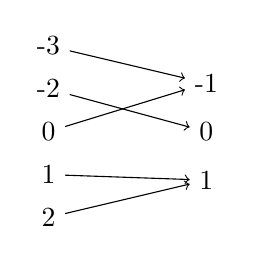
\begin{tikzpicture}[scale=.5]
		\node (n3) {-3};
		\node[below=2pt of n3] (n2) {-2};
		\node[below=2pt of n2] (o) {0};
		\node[below=2pt of o] (p1) {1};
		\node[below=2pt of p1] (p2) {2};
		
		\node[right=45pt of o] (o2) {0};
		\node[above=4pt of o2] (nn1) {-1};
		\node[below=4pt of o2] (pp1) {1};
		
		\draw[->] (n3) -- (nn1);
		\draw[->] (n2) -- (o2);
		\draw[->] (o) -- (nn1);
		\draw[->] (p1) -- (pp1);
		\draw[->] (p2) -- (pp1);
	\end{tikzpicture}
	For this mapping diagram, the domain would be $D=\{-3, -2, 0, 1, 2\}$ and the range would be $R=\{-1, 0, 1\}$
	\subsubsection{Functions}
	A function can only assign one element from the set of Y values (the range) to each element from the set of X values (the domain). $y=f(x)$ where $x$ is the argument or the input of the function and $y$ is the value or the output of the function.\\
	Using the function $f(x)=(x-1)^2$:
	\begin{itemize}
		\item $f(0)=1$
		\item $f(\frac{1}{2})=\frac{1}{4}$
		\item $f(a+2)=a^2+2a+1$
	\end{itemize}
	\subsubsection{Graph}
	The graph of a function $f$ is the graph of the set of ordered pairs $(x, y)$ where $y=f(x)$.\\
	The graph of the function defined by a set of ordered pairs $f=\{(2, 3), (0, -2), (-4, 3), (4, 0), (-3, -3)\}$:\\
	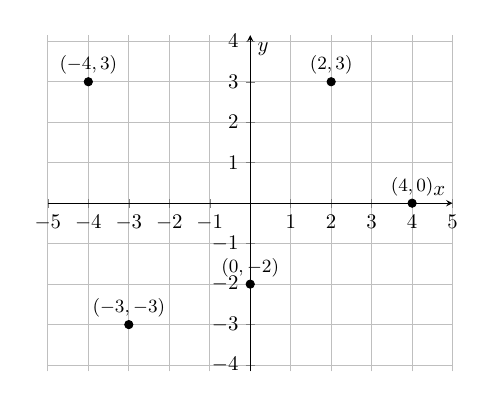
\begin{tikzpicture}[scale=.75]
		\begin{axis}[
			scatter/classes={a={draw=red,fill=red}},
			axis y line*=left,
			axis x line*=bottom,
			grid=both,
			ymin=-4,
			xmin=-5,
			ymax=4,
			xmax=5,
			axis equal,
			axis lines=middle,
			xlabel=$x$,
			ylabel=$y$,
			xtick distance=1,
			ytick distance=1
		]
		%TODO: Fix this so that the points are still red (Change the label something)
		\addplot[mark=*,scatter,only marks,scatter src=explicit symbolic,nodes near coords={\labelz}, visualization depends on={value {\small$(\thisrowno{0}, \thisrowno{1})$}\as\labelz}]
		table[meta=label] {
			x y label
			2 3 a
			0 -2 a
			-4 3 a
			4 0 a
			-3 -3 a
		};
		\end{axis}
	\end{tikzpicture}
	\subsubsection{Vertical Line Test}
	All functions are relations but not all relations are functions. A graph represents a function if every vertical line intersects the graph in at most one point.\\
	The set of ordered pairs $\{(0, 0), (-1, -1), (2, 2), (1, -1)\}$ represents a function, while the set of ordered pairs $\{(2, 3), (-1, 3), (2, -2), (-3, -1)\}$ does not.
	%TODO: The actual graphs with vertical lines
	\subsubsection{Domain and Range}
	The domain of a function $f$ is the set of all real numbers $x$ for which $f(x)$ is defined. The range of a function $f$ is the set of all real numbers $y$ for which $y=f(x)$  is defined.\\
	The domain and range for the set of ordered pairs $\{(-2, 0), (-1, 1), (0, -1), (1, 0)\}$ is $D=\{-2, -1, 0, 1\}$ and $\{-1, 0, 1\}$. The domain and range for the set of ordered pairs $\{(-1, 0), (0, 1), (1, 0), (3, 1), (7, 0)\}$ is $D=\{-1, 0, 1, 3, 7\}$ and $\{0, 1\}$.
	%TODO: Graphs with domain and range
	\subsubsection{Restrictions}
	Division by 0 is undefined, so the denominator of a function cannot equal 0. Square roots are undefined for negative numbers and square roots cannot be negative, so for $f(x)=\sqrt{x}$, $x\geq0$ and $f(x)\geq0$. Squares cannot be negative so for $f(x)=x^2$, $f(x)\geq0$.\\
	For $y=(x-1)^2-3$:
	\begin{itemize}
		\item $D=\{x\in R\}$
		\item $R=\{y\in R\mid y\geq-3\}$
	\end{itemize}
	For $y=2+\sqrt{x-3}$:
	\begin{itemize}
		\item $D=\{x\in R\mid x\geq3\}$
		\item $R=\{y\in R\mid y\geq2\}$
	\end{itemize}
	For $y=\frac{x-2}{x+2}$: $=\frac{x+2-4}{x+2}$ $=1-\frac{4}{x+2}$
	\begin{itemize}
		\item $D=\{x\in R\mid x\neq-2\}$
		\item $R=\{y\in R\mid y\neq1\}$
	\end{itemize}
	\subsection{Exploring Absolute Value}
	\subsubsection{Absolute Value}
	The absolute value $|x|$ of a real number $x$ is the distance between $x$ and 0.\\
	For example, $|5|=|-5|=5$ and $\left|2-\left|-3\right|\right|$.
	\subsubsection{Definition of Absolute Value}
	The absolute value $|x|$ is defined by:
	\[|x|=\begin{cases}
		x&\text{if }x\geq0\\
		-x&\text{if }x<0
	\end{cases}\]
	Therefore:
	\[|x-3|=\begin{cases}
		x-3&\text{if }x\geq3\\
		-x+3&\text{if }x<3
	\end{cases}\]
	\subsubsection{Properties of Absolute Value}
	Absolute values have the following properties:
	\begin{itemize}
		\item $|a|=|-a|$
		\item if $|a|=0$, $a=0$
		\item $|ab|=|a||b|$
		\item $\left|\frac{a}{b}\right|=\frac{|a|}{|b|}$
		\item $|a+b|\leq|a|+|b|$ (proved by triangle inequality)
	\end{itemize}
	For example, $\left|\frac{-2x}{3y}\right|\left|\frac{-2y}{3x}\right|=\frac{|-2||x|}{|3||y|}\cdot\frac{|-2||y|}{|3||x|}=\frac{4}{9}$. Also, $|-3x|-|-x|-|x|=3|x|-|x|-|x|=|x|$
	\subsubsection{Distance between two numbers}
	The distance between two numbers $a$ and $b$ on the number line can be represented by $|a-b|$.
	For example, in the equation $|x-3|=|5-x|$, $x$ would represent a number that is the same distance from 3 as is to 5. This can be solved algebraically:
	\begin{align*}
		&&x-3&=\pm(5-x)\\
		\text{Ca}&\text{se 1}&&&\text{Ca}&\text{se 2}\\
		x-3&=5-x&&&x-3&=x-5\\
		2x&=8&&&-3&=-5\\
		x&=4&&&\text{No }&\text{Solution}\\
		&&\therefore{}&x=4
	\end{align*}
	\subsubsection{Equations}
	If $E(x)$ is an algebraic expression containing the variable $x$, the equation $|E(x)|=a; a\geq0$ can be solved from isolating $x$ from the equation $E(x)=\pm a$\\
	For example, from the equation $\left|2-\frac{2x+1}{2x-1}\right|=1$:
	\begin{align*}
		\left|\frac{(4x-2)-(2x+1)}{2x-1}\right|&=1;x\neq\frac{1}{2}\\
		\frac{2x-3}{2x-1}&=\pm1\\
		\begin{cases}
			2x-3\\
			2x-3
		\end{cases}&
	\end{align*}
	\subsection{Properties of Graphs of Functions}
	\subsection{Sketching Graphs of Functions}
	\subsubsection{Parent Functions}
	Parent functions are functions in ``simplest form''. Parent functions may be used to create more complicated functions. For example, the function $g(x)=-2\dfrac{1}{(x-1)^2}+3$ is a transformation of the parent function $f(x)=\dfrac{1}{x^2}$. Parent functions can be graphed with key point. For example, five key points of the parent function $f(x)=\sqrt[3]{x}$ are $(-8, -2)$, $(-1, -1)$, $(0, 0)$, $(1, 1)$, and $(8, 2)$.
	%TODO: maybe some examples?
	\subsubsection{Transformations}
	Given a parent function $f(x)$, we can create new functions using the transformations $g(x)=af(b(x-c))+d$. The graph is:
	\begin{itemize}
		\item vertically stretched by $|a|$
		\item reflected on the $x$ axis if $a<0$
		\item horizontally stretched by $\left|\dfrac{1}{b}\right|$
		\item reflected on the $y$ axis if $b<0$
		\item shifted to the right by $c$
		\item shifted up by $d$
	\end{itemize}
	\subsubsection{Mapping Formulas}
	By comparing the parent function $y=f(x)$ and the image (new) function $y'=af(b(x'-c))+d$, we get:
	\[\begin{cases} 
	y'=ay+d\\
	x'=\frac{x}{b}+c
	\end{cases}\]
	%TODO: examples
	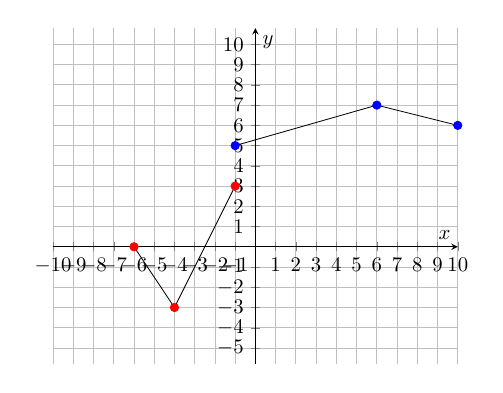
\begin{tikzpicture}[scale=.75]
		\begin{axis}[
			scatter/classes={f={draw=red,fill=red},g={draw=blue,fill=blue}},
			axis y line*=left,
			axis x line*=bottom,
			grid=both,
			ymin=-5,
			xmin=-10,
			ymax=10,
			xmax=10,
			axis equal,
			axis lines=middle,
			xlabel=$x$,
			ylabel=$y$,
			xtick distance= 1, ytick distance = 1
		]
		\addplot[scatter,scatter src=explicit symbolic]
			table[meta=label] {
				x y label
				-6 0 f
				-4 -3 f
				-1 3 f
				
				-1 5 g
				6 7 g
				10 6 g
			};
		\end{axis}
	\end{tikzpicture}\\
	To write the function $g(x)$ in the form $g(x)=af(b(x-c))+d$, we have to solve for all 4 of the variables, with 4 equations from the graph. We can know which point corresponds to which point because each segment will have the same proportions. Therefore, we can use these four equations (there are other possibilities): \[\]
	\subsubsection{Domain and Range}
	After transformations, the domain and range may be changed. The mapping formulas can be used to calculate the new ones.\\
	For example: A function with domain $D=(-1,3]$ and range $R=[2,\infty)$ is transformed into a new function $g(x)=-2f(2x-3)+4$. $a=-2$, $b=2$, $c=\frac{3}{2}$, $d=4$. The domain would be shifted to $\left(\frac{-1}{2}+\frac{3}{2}, \frac{3}{2}+\frac{3}{2}\right]=(1,3]$ and the range would be shifted to $\left[-2(2)+4, -2(\infty)+4\right)=[0, -\infty)$
	\subsection{Inverse Relations}
	\subsubsection{Inverse Relation}
	For any relation there is an inverse relation obtained by switching the $x$ and $y$ values for all the elements of the original relation. The inverse relation of a relation $r$ is denoted by $r^{-1}$. A 1:1 function is a function where the inverse is also a function; it passes both the vertical and horizontal line tests.\\
	The inverse relation of the relation $r=\{(1, 2), (1, 0), (-2, 1), (0, 2)\}$ is $r^{-1}=\{(2, 1), (0, 1), (1, -2), (2, 0)\}$
	\subsubsection{Symmetry}
	The graph of a relation and the graph of its inverse relation are symmetrical about the line $y=x$.
	%TODO: graph
	\subsubsection{Corresponding Key Points}
	A point $P(x, y)$ on the relation $r$ corresponds to the point $P'(y, x)$ on the inverse relation $r^{-1}$. The points $P$ and $P'$ are symmetrical about the line $y=x$.
	%TODO: graph
	\subsubsection{Domain and Range}
	The domain of the inverse relation $r^{-1}$ is the same as the range of the range of the relation $r$; $D_{r^{-1}}=R_r$. The range of the inverse relation $r^{-1}$ is the same as the domain of the range of the relation $r$; $R_{r^{-1}}=D_r$.\\
	A relation $r$ is given by the following mapping diagram:\\
	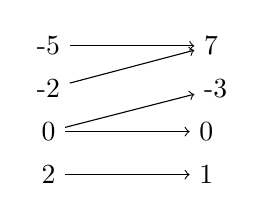
\begin{tikzpicture}[scale=.5]
		\node (n5) {-5};
		\node[below=2pt of n5] (n2) {-2};
		\node[below=2pt of n2] (o) {0};
		\node[below=2pt of o] (p2) {2};
	
		\node[right=45pt of n5] (p7) {7};
		\node[right=45pt of n2] (n3) {-3};
		\node[right=45pt of o] (o2) {0};
		\node[right=45pt of p2] (p1) {1};
	
		\draw[->] (n5) -- (p7);
		\draw[->] (n2) -- (p7);
		\draw[->] (o) -- (n3);
		\draw[->] (o) -- (o2);
		\draw[->] (p2) -- (p1);
	\end{tikzpicture}
	The domain of $r$ is $D={-5, -2, 0, 2}$ and the range is $R={-3, 0, 1, 7}$.
	The domain of $r^{-1}$ is $D={-3, 0, 1, 7}$ and the range is $R={-5, -2, 0, 2}$.
	\subsubsection{Inverse Relation of a Function}
	Any function is a relation. So, any function $f$ has an inverse relation $f^{-1}$.
	\subsection{Piecewise Functions}
	\subsubsection{Piecewise-Defined Functions}
	A piecewise-defined function requires more than one formula to explicitly define the function. Each formula is defined on a different interval. The domain of a piecewise-defined function is the union of all the intervals used to define the function.\\
	For example, the function $y=|x-2|$ can be rewritten as $y=\begin{cases}
		x-2&\text{if }x\geq2\\
		-x+2&\text{if }x<2
	\end{cases}$\\
	The heaviside function can be represented as $h(x)=\begin{cases}
		1&\text{if }x\geq0\\
		0&\text{if }x<0
	\end{cases}$\\
	%Graph
	%Step function
	The Dirichlet function can represented as $d(x)=\begin{cases}
		1&\text{if }x\text{ is rational}\\
		0&\text{if }x\text{ is irrational}
	\end{cases}$. Sometimes, $\frac{1}{b}$ (where the rational $x$ is represented as $\frac{a}{b}$) is used instead of 1.\\
	The function $f(x)=1-|x+1|-|x+2|$ can be rewritten as $f(x)=\begin{cases}
		x+x+1+x+2=3x+3&x<-2\\x+x+1-x-2=x-1&-2\leq x<-1\\x-x-1-x-2=-x-3&x\geq-1
	\end{cases}$\\
	$f(x)=\begin{cases}
		1&\text{if }x>0\\
		-1&\text{if }x<0
	\end{cases}$
	
	%more examples
	\subsubsection{Continuity}
	The graph of a continuous function can be drawn without lifting your pencil from the paper. A continuous function has no holes, finite gaps, or infinite breaks.\\
	For example, to calculate a value of $c$ where the function is continuous: $f(x)=\begin{cases}
		x+c&\text{if }x<2\\
		cx^2+1&\text{if }x\geq2
	\end{cases}$
	\begin{align}
		2+c&=c(2)^2+1\\
		2+c&=4c+1\\
	\end{align}
	%$sometihing belongs here$
	\subsubsection{Absolute Value}
	The absolute value of a function is defined by
	\[|f(x)|=\begin{cases}
		f(x)&\text{if }f(x)\geq0\\
		-f(x)&\text{if }f(x)<0
	\end{cases}\]
	\setcounter{section}{9}
	\setcounter{subsection}{0}
	\subsection{asdf}
	\subsection{asdf}
	\subsection{asdf}
	\subsection{asdf}
	\subsection{Composition of Functions}
	\subsubsection{Composition of Functions}
	\setcounter{section}{3}
	\setcounter{subsection}{0}
	\tsection{Unit 2: Polynomial Functions}
	\subsection{Exploring Polynomial Functions}
	\subsubsection{Polynomial Functions}
	A polynomial function $f(x)$ is defined by: $f(x) = a_nx^n+a_{n-1}x^{n-1}+\ldots+a_2x^2+a_1x+a_0$, where:
	\begin{itemize}
		\item $a_n$, $a_{n-1}$, \ldots, $a_2$, $a_1$, $a_0$ are real numbers called the coefficients of the polynomial function
		\item $a_n$ is called the leading coefficient
		\item $a_nx^n$ x is called the leading term
		\item $a_0$ is called the constant term
		\item $n$ is a non-negative integer that gives the degree of the polynomial function
		\item the degree of a polynomial function $n$ is the largest exponent of $x$
	\end{itemize}
	\subsection{Characteristics of Polynomial Functions}
	\subsubsection{End Behavior}
	For very large $x$ ($x\to\infty$ or $x\to-\infty$), the graph of the polynomial function will resemble the graph of the leading term $a_nx^n$\\
	For example, if $a_n>0$ and $n$ is even, as $x\to\infty$, $y\to\infty$, and as $x\to-\infty$, $y\to\infty$, or if $a_n<0$ and $n$ is odd, $x\to\infty$, $y\to-\infty$, and as $x\to-\infty$, $y\to\infty$.
	\subsubsection{Symmetry}
	A polynomial function is even if all the powers of $x$ are even, or odd if all the powers of $x$ are odd.\\
	For example, $x-x^3+2x^5$ is odd, $2-x^2+3x^6$ is even, and $1+x-x^3+3x^4$ is neither.
	\subsubsection{Zeroes and the Fundamental Theorem of Algebra}
	\begin{itemize}
		\item A polynomial function of degree $n$ has $n$ zeroes, real or complex
		\item If the coefficients of the polynomial function are real numbers, the complex zeroes come in conjugate pairs; there are an even number of complex zeroes
		\item The number of real zeroes is at most $n$, but these zeroes may be coincident
		\item A polynomial function with an even degree may have no real zeroes
		\item A polynomial function with an odd degree must have at least one real zero
	\end{itemize}
	\subsubsection{Turning Points}
	A turning point is the point where increasing changed to decreasing or vice versa. A polynomial function of $n$ has at most $n-1$ turning points
	\subsubsection{Extrema Points}
	Extrema is the plural of extremum. Extremum is either a minimum or maximum, and may be local or global. Each turning point is a local extrema point. A polynomial function with an even degree has either a global minimum or global maximum point. A polynomial function with an odd degree has neither a global maximum or a global minimum point.
	\subsection{Polynomial Functions in Factored Form}
	\subsubsection{Simple Zeroes}
	Some polynomial functions can be factored into the form $f(x)=a_n(x-x_1)(x-x_2)\dots(x-x_{n-1})(x-x_n)$ where $x_1, x_2, \dots, x_{n-1}, x_n$ are $n$ distinct real numbers and are the zeroes of the function
	\subsubsection{Repeated Zeroes}
	Some polynomial functions can be factored into the form 
	\subsection{Transformations of Cubic and Quartic Functions}
	\subsubsection{Cubic Funcitons}
	%The graph
	Cubic functions have the parent function $f(x)=x^3$, and after transformations, may be written as $f(x)=a[b(x-c)]^3+d$
	\subsubsection{Quartic Functions}
	%The graph
	Cubic functions have the parent function $f(x)=x^4$, and after transformations, may be written as $f(x)=a[b(x-c)]^4+d$
	\subsubsection{Power Function(Real Exponent)}
	\subsubsection{Power Function(Rational Exponent)}
	\subsection{Dividing Polynomials}
	\subsubsection{Division of Natural Numbers}
	If $D$ and $d\neq0$ are two natural numbers, then there are unique numbers $q$ and $r$ such that the relation (called the division statement) $\frac{D}{d}=\frac{r}{d}$ or $D=dq+r$ is true; where $0\leq r<d$.
	\begin{itemize}
		\item $D$ is called the dividend
		\item $d$ is called the divisor
		\item $q$ is called the quotient
		\item $r$ is called the remainder
	\end{itemize}
	If the remainder is 0, then $D$ is divisible by $d$, or $d$ divides evenly into $D$.
	\subsubsection{Division of Polynomials}
	If $D(x)$ and $d(x)$ are two polynomial functions, then there are two unique polynomial functions $q(x)$ and $r(x)$ such that the relation $\frac{D(x)}{d(x)}=\frac{r(x)}{d(x)}$ or $D=d(x)q(x)+r(x)$ is true; where $0\leq\deg r<\deg d$
	\subsection{Factoring Polynomials}
	\subsubsection{The Remainder Theorem}
	If a polynomial $P(x)$ is divided by $x-b$, then the remainder is $P(b)$; Proof:
	\begin{align*}
		P(x)&=q(x)(x-b)+r(x)\\
		P(b)&=q(b)(b-b)+r(b)\\
		&=q(b)(0)+r(b)\\
		&=r(b)
	\end{align*}
	For example, when $x^3-kx^2+17x+6$ is divided by $x-3$ and the remainder is 12, you can find the value of k by equating $P(3)=12=3^3-k3^2+17(3)+6=27-9k+51+6=84-9k$, so $9k=72; k=8$
	\subsubsection{The Remainder Theorem, Part II}
	If a polynomial $P(x)$ is divided by $ax-b$, then the remainder is $P(\frac{b}{a})$; Proof:
	\begin{align*}
		P(x)&=q(x)(ax-b)+r(x)\\
		P\left(\frac{b}{a}\right)&=q\left(\frac{b}{a}\right)\left(a\left(\frac{b}{a}\right)-b\right)+r\left(\frac{b}{a}\right)\\
		&=q\left(\frac{b}{a}\right)\left(b-b\right)+r\left(\frac{b}{a}\right)\\
		&=q\left(\frac{b}{a}\right)\left(0\right)+r\left(\frac{b}{a}\right)\\
		&=r\left(\frac{b}{a}\right)
	\end{align*}
	\subsubsection{The Factor Theorem}
	A polynomial $P(x)$ has $x-b$ as a factor if and only if $P(b)=0$.\\
	For example: $x+2$ is a factor of $x^3+5x^2+2x-8$ because $(-2)^3+5(-2)^2+2(-2)-8=-8+20-4-8=0$\\
	%Note: you can use the $\pm$ factors of the last term to find factors
	\subsubsection{Integral Zero Theorem}
	If $x=b$ is an integral zero of the polynomial $P(x)$ with integral coefficients, then $b$ is a factor (divisor) of the constant term, $a_0$.
	For example
	\subsection{Factoring Sums or Differences of Cubes and Powers}
	\subsubsection{Difference of Two Cubes}
	The difference of cubes identity is: $a^3-b^3=(a-b)(a^2+ab+b^2)$\\
	For example: you can factor $x^3-8$ into $(x-2)(x^2+2x+4)$, or $\frac{x^3}{27}-125$ into $(\frac{x}{3}-5)(\frac{x^2}{9}+\frac{5x}{3}+25)$
	\subsubsection{Sum of Two Cubes}
	The sum of cubes identity is: $a^3+b^3=(a+b)(a^2-ab+b^2)$\\
	For example: you can factor $x^3+1$ int $(x+1)(x^2-x+1)$, or $\frac{x^3}{64}+\frac{8}{27}$ into $(\frac{x}{4}+\frac{2}{3})(\frac{x^2}{16}-\frac{x}{6}+\frac{4}{9})$
	\subsubsection{Difference of Two Powers}
	For any natural number $n$, the following identity is true: \[a^n-b^n=(a-b)(a^{n-1}+a^{n-2}b+a^{n-3}b^2+\dots+a^2b^{n-3}+ab^{n-2}+b^{n-1})\]
	For example: $x^4-16$ can be factored into $(x^2-4)(x^2+4)=(x+2)(x-2)(x^2+4)$
	\subsubsection{Sum of Two Powers}
	For any natural odd number $n$, the following identity is true: \[a^n+b^n=(a+b)(a^{n-1}-a^{n-2}b+a^{n-3}b^2-\dots-a^2b^{n-3}+ab^{n-2}-b^{n-1})\]
	For example: $sdf$ can be factored into $asdf$\\
	%more examples
	General Example: Given that $a-b=4$ and $ab=2$, to find $a^3-b^3$:\\
	\begin{align*}
		a^3-b^3&=(a-b)(a^2+ab+b^2)\\
		(a-b)^2&=a^2-2ab+b^2\\
		\therefore a^3-b^3&=(4)(4^2+3(2))=4(16+6)=4(22)=88
	\end{align*}
	\setcounter{section}{4}
	\setcounter{subsection}{1}
	\subsection{Solving Linear Polynomial Equations}
	\subsubsection{Fundamental Theorem of Algebra}
	\begin{flalign*}
		\renewcommand\arraystretch{1.5}
		\begin{array}{rrrrrr}
			\multicolumn{1}{r|}{2} & 1 & -4 & 7 & 0 & -12\\
			\multicolumn{1}{r|}{}& & 2 & -4 & 6 & 12\\\cline{2-6}
			\multicolumn{1}{r|}{-1}& 1 & -2 & 3 & 6 & 0\\
			\multicolumn{1}{r|}{}& & -1 & 3 & -6\\\cline{2-5}
			& 1 & -3 & 6 & 0
		\end{array}
	\end{flalign*}
	\subsubsection{asdf}
	\subsubsection{asdf}
	\subsubsection{Real Zeroes}
	If $a+b\sqrt{c}$ where $a$, $b$, and $c$ are rational numbers and $c>0$ is a zero of a polynomial with integral coefficients, then $a-b\sqrt{c}$ is also a zero of this polynomial
	\subsubsection{Technology}
	In some cases, the real zeroes of a polynomial equation may only be found using technology. For example, you can use technology to find the real zeroes of $x^3+x-1$: a,b, c
	\subsection{Solving Polynomial Inequalities}
	\subsection{Solving Polynomial Inequalities}
	\subsubsection{Sign Chart Method}
	To solve $x(x-1)\leq0$
	\begin{flalign*}
		\renewcommand\arraystretch{1.3}
		\begin{array}{r|ccccc}
		x     & &0& &1& \\\hline
		x     &-&0&+&+&+\\\hline
		x-1   &-&-&-&0&+\\\hline
		x(x-1)&+&0&-&0&+\\\hline
		\end{array}\\
		x\in[0, 1]
	\end{flalign*}
	To solve $(x^2-x-2)(x^2+1)(x-3)^3\geq0$, you can factor to $(x-2)(x+1)(x^2+1)(x-3)^3\geq0$
	\begin{flalign*}
	\renewcommand\arraystretch{1.3}
		\begin{array}{r|ccccccc}
			x      & &-1& &2& &3& \\\hline
			x-2    &-&- &-&0&+&+&+\\\hline
			x+1    &-&0 &+&+&+&+&+\\\hline
			(x-3)^3&-&- &-&-&-&0&+\\\hline
			f(x)   &-&0 &+&0&-&0&+\\\hline
		\end{array}\\
		x\in[-1, 2]\cup[3,\infty)
	\end{flalign*}
	\subsubsection{Graphical Method}
	You can graph the polynomial and visualize the inequality.\\
	For example, you can look at the graph of $x(x-1)(x+2)>0$ and see where it is greater than 0
	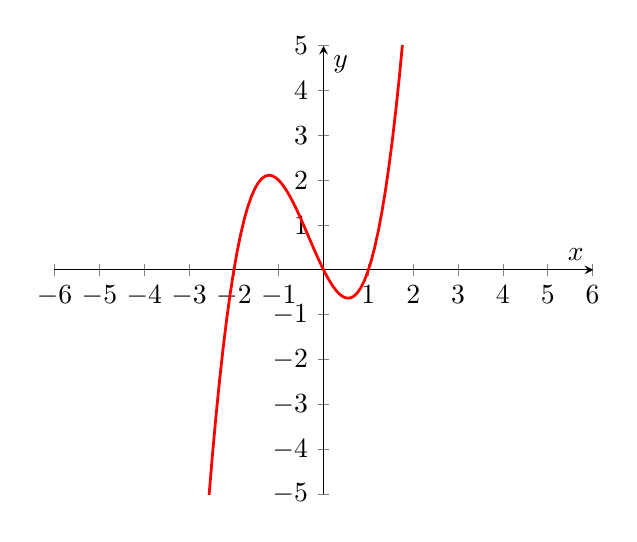
\begin{tikzpicture}
		\begin{axis}[
			axis y line*=left,
			axis x line*=bottom,
			ymin=-5,
			xmin=-4,
			ymax=5,
			xmax=4,
			axis equal,
			axis lines=middle,
			xlabel=$x$,
			ylabel=$y$,
			xtick distance=1,
			ytick distance=1,
		]
		\addplot+[<->, mark=none, red, samples=128, line width=1pt]{x*(x-1)*(x+2)};
		\end{axis}
	\end{tikzpicture}
	\subsubsection{Algorithm to Solve Polynomial Inequalities}
	To solve an inequality involving a polynomial expression:
	\begin{itemize}
		\item Move all terms to one side of the inequality
		\item Factor the polynomial
		\item Use a sign chart or graphical method to find the [sign] of the polynomial
		\item Write the solution
	\end{itemize}
	\subsubsection{Technology}
	If you cannot factor the polynomial, use technology to find the solution
	\tsection{Unit 3: Rational Functions}
	\setcounter{section}{5}
	\setcounter{subsection}{1}
	\subsection{Graphs of Reciprocal Functions}
	\subsubsection{General Rules}
	For a function $f(x)$ and its reciprocal $g(x)=\frac{1}{f(x)}$, there are some general rules
	\begin{itemize}
		\item If the function $f(x)$ has a zero at $x=a$, the reciprocal function $g(x)$ has a vertical asymptote at $x=a$, and vice versa
	\end{itemize}
	\subsection{Rational Functions}
	\subsubsection{Rational Functions}
	A rational function is in the form $f(x)=\frac{P(x)}{Q(x)}$ where $P(x)$ and $Q(x)$ are polynomial functions.
	\subsubsection{Domain}
	The domain of a rational function is determined by $Q(x)\neq0$.\\
	For example, $f(x)=\frac{x^2-1}{x-1}=\frac{(x+1)(x-1)}{x-1}=x+1$ where $D=\{x\in\mathbb{R}\mid x\neq1\}$.\\
	For $f(x)=\frac{x^2-x}{6x^3+x^2-2x}=\frac{x(x-1)}{x(2x-1)(3x+2)}$ and $d=\{x\in\mathbb{R}\mid x\neq0, \frac{1}{2}, -\frac{2}{3}\}$. There is a hole at $(0, \frac{1}{2})$, and vertical asymptotes at $x=\frac{1}{2}$ and $x=-\frac{2}{3}$. As $x\to-\frac{2}{3}^-$, $y\to-\infty$, and $x\to-\frac{2}{3}^+$, $y\to\infty$. As $x\to\frac{1}{2}^-$, $y\to\infty$, and $x\to\frac{1}{2}^+$, $y\to-\infty$. You can use the leading terms to find the end behavior and find the horizontal asymptote at $y=0$\\
	\[\frac{{P(x)}}{Q(x)}=\frac{a_nx^n+a_{n-1}x^{n-1}+\dots+a_1x_1+a_0}{b_mx^m+b_{m-1}x^{m-1}+\dots+b_1x_1+b_0}=\frac{\infty}{\infty}=\frac{a_nx^n\left(1+\frac{a_{n-1}}{a_nx}+\dots+\frac{a_1}{a_nx^{n-1}}+\frac{a_0}{a_nx^n}\right)}{{b_mx^m\left(1+\frac{b_{m-1}}{b_mx}+\dots+\frac{b_m}{b_mx^{m-1}}+\frac{b_0}{b_mx^m}\right)}}\]
	\[\lim_{|x|\to\infty}f(x)=\lim_{|x|\to\infty}\frac{a_nx^n}{b_mx^m}
	\begin{cases}\begin{aligned}
		&n=m&&y=\frac{a_n}{b_m}&&\text{HA}\\
		&n<m&&y=0&&\text{HA}\\
		&n>m&&&&\text{no HA, becomes unbounded}\\
		&n=m+1&&&&\text{oblique asymptote, from quotient}
	\end{aligned}\end{cases}\]
	\subsection{Solving Rational Equations}
	\subsubsection{Rational Equations}
	To solve a rational equation:
	\begin{itemize}
		\item State restrictions
		\item Find the least common denominator (LCD)
		\item Multiply so that all terms are over the LCD
		\item Solve the polynomial equation
		\item Verify with restrictions
	\end{itemize}
	For example: to solve $\frac{x}{x-2}-\frac{2}{x+3}=\frac{10}{x^2+x-6}$, you can factor it into $\frac{x}{x-2}-\frac{2}{x+3}=\frac{10}{(x-2)(x+3)}$. You find the restrictions, $x\neq2,-3$. Then, the least common denominator is $(x-2)(x+3)$. After you multiply, you end up with $\frac{x(x+3)}{(x-2)(x+3)}-\frac{2(x-2)}{(x+3)(x-2)}=\frac{10}{(x-2)(x+3)}$. This is equal to $\frac{x^2+3x-2x+4}{(x+3)(x-2)}=\frac{10}{(x-2)(x+3)}$, which is $x^2+x+4=10$, $x^2+x-6=0$, $(x-2)(x+3)=0$. The solutions for this equation are 2 and $-3$, but since the restrictions for the original equation are $x\neq2,-3$, there are no solutions.
	\subsubsection{Cross Multiplication}
	A rational equation of the form $\frac{P(x)}{Q(x)}=\frac{R(x)}{S(x)}\Leftrightarrow P(x)S(x)=Q(x)R(x)$\\
	For example, to solve $\frac{x-1}{2x+3}=\frac{x+2}{3x-2}$, you can change it to $(x-1)(3x-2)=(x+2)(2x+)$
	\subsubsection{Shortcut}
	\subsection{Solving Rational Inequalities}
	\subsubsection{Rational Inequalities}
	\subsection{Rates of Change of Rational Functions}
	\subsubsection{Average Rate of Change}
	The average rate of change (ARC) over an interval $[x_1, x_2]$, is defined as $\frac{f(x_2)-f(x_1)}{x_2-x_1}$, or $\frac{\Delta y}{\Delta x}$. This is the same as the slope of the secant line from $(x_1, f(x_1))$ to $(x_2, f(x_2))$.
	\subsubsection{Instantaneous Rate of Change}
	The instantaneous rate of change (IRC) is defined as $x_1\rightarrow x_2$, the same function. However, since $x_1$ is approaching $x_2$, it would become $\lim_{x_1\to x_2}\frac{f(x_2)-f(x_1)}{x_2-x_1}$. Or, if you use $h$ as the difference between the two $x$ values, $\lim_{h\to 0}\frac{f(x+h)-f(x)}{h}$. \\
	For example, to calculate the IRC of Newton's Serpentine $f(x)=\frac{4x}{x^2+1}$ at $x=0$:
	\begin{align*}
		\text{IRC}&=\lim_{h\to 0}\frac{f(0+h)-f(0)}{h}\\
		&=lim_{h\to 0}\frac{\frac{4h}{h^2+1}}{h}\\
		&=lim_{h\to 0}\frac{4}{h^2+1}\\
		&=4
	\end{align*}
	To calculate the instantaneous rate of change for any point in the graph, you can calculate the difference quotient ($DQ$), $\frac{f(x+h)-f(x)}{h}$, then use $\lim_{h\to 0}$ on it.
	\begin{align*}
		DQ&=\frac{f(x+h)-f(x)}{h}\\
		&=\frac{\frac{f(x+h)}{(x+h)^2+1}-\frac{4x}{x^2+1}}{h}\\
		&=\frac{4(x+h)(x^2+1)-4x(x^2+2xh+h^2+1)}{h(x^2+1)\left((x+h)^2+1\right)}\\
		&=\frac{4x^3+4x+4hx^2+4h-4x^3-8x^2h-4xh^2-4x}{h(x^2+1)\left((x+h)^2+1\right)}\\
		&=\frac{-4x^2h+4h-4xh^2}{h(x^2+1)\left((x+h)^2+1\right)}\\
		&=\frac{-4x^2+4-4xh}{(x^2+1)\left((x+h)^2+1\right)}
	\end{align*}
	Then, the IRC = $\lim\limits_{h\to 0}DQ$, so you can sub $h=0$ into $DQ$, to end up with IRC $=\frac{-4x^2+4}{(x^2+1)^2}$\\
	For $f(x)=\frac{x-2}{x-5}$:\\
	\begin{align*}
		DQ&=\frac{\frac{x+h-2}{x+h-5}-\frac{x-2}{x-5}}{h}
	\end{align*}
	\tsubsection{AP Component: Partial Fraction Decomposition}
	Partial Fraction Decomposition is the inverse operation of addition or subtraction of fractions. For example, you can decompose $\frac{2x}{x^2-1}=\frac{2x}{(x+1)(x-2)}$ into $\frac{2x}{(x+1)(x-2)}=\frac{a}{x-1}+\frac{b}{x+1}=\frac{a(x+1)+b(x-1)}{(x+1)(x-2)}$. Since they have the same denominators, $2x=a(x+1)+b(x-1)$. Since each degree of x must have the same value on both sides, the coefficient of $x^1$, 2, mus equal $a+b$, and the coefficient of $x^0$, 0, must equal $a-b$. We can solve this system of equations to obtain $a=1$ and $b=1$.\\
	To solve 
	\tsection{Unit 4: Exponential and Rational Functions}
	\setcounter{section}{8}
	\setcounter{subsection}{0}
	\subsection{Exploring the Logarithmic Function}
	\subsubsection{Logarithmic Functions}
	$b^x$ is the exponential function, while $x^n$ is the power function. For the exponential function, the base, $b$, is defined as $b>0$ and $b\neq1$, to get a useful graph. You know you have an exponential function if the $1,2,3\dots n$th differences are all proportional.%example maybe
	For exponential functions, the domain is $x\in\mathbb{R}$, while the range is $y\in\mathbb{R}\mid y>0$. They have a horizontal asymptote at $y=0$, but no vertical asymptote. There is a y-intercept at $y=1$, but there is no x-intercept. Their y-intercept is called an invariance point, as it doesn't change based on the base. Exponential functions are one-to-one functions, so their inverse is also a function.\\
	Their inverse is the log function $f(x)=\log_bx$. They have an invariance point at (1, 0). The domain is $x\in\mathbb{R}\mid x>0$, and the range is $y\in\mathbb{R}$.  They have no y-intercept, but they have an x-intercept at $x=1$. They have a vertical asymptote at $y=0$, but no horizontal asymptote. The limits of the vertical asymptote are $\lim\limits_{x\to0^+}f(x)=-\infty$ if $b>1$, and $\lim\limits_{x\to0^+}f(x)=\infty$ if $0<b<1$.
	\subsection{ASDf}
	\tsubsection{AP Component: Hyperbolic Functions}
	\tsubsection{AP Component: Inverse of Hyperbolic Functions}
	To get the equation of the inverse of $\sinh x$, you can sub $x$ and $y$ into the definition of $\sinh x$:
	\begin{align*}
		x&=\sinh y&\\
		&=\frac{e^y-e^{-y}}{2}\\
		2x&=e^y-e^{-y}\\
		e^y-e^{-y}-2x&=0\\
		e^{2y}-2xe^y-1&=0\\
		\text{After plugging into quadratic formula: }e^y&=\frac{-(-2x)\pm\sqrt{(2x)^2-4(1)(-1)}}{2(1)}\\
		&=\frac{2x\pm\sqrt{4x^2+4}}{2}\\
		&=\frac{2x\pm\sqrt{4(x^2+1)}}{2}\\
		&=x\pm\sqrt{x^2+1}\\
		\because e^y>0\therefore&\text{ we can only take }x+\sqrt{x^2+1}\\
		\sinh^{-1}x&=\ln\left(x+\sqrt{x^2+1}\right)
	\end{align*}
	\tsection{Unit 5: Rates of Change and Derivatives}
	\setcounter{section}{2}
	\setcounter{subsection}{1}
	\tsubsection{AP Component: Derivative Functions and First Principles}
	\subsubsection{Derivative Functions}
	Given a function $y=f(x)$, the \textit{derivative function} of $f$ is a new function , $f'$ ($f$ prime), defined at $x$ by:
	\[f'(x)=\lim_{h\to0}\frac{f(x+h)-f(x)}{h}\]
	\subsubsection{Differentiability}
	A function $y=f(x)$ is called \textit{differentiable} at $x$ if $f'(x)$ exists. A function $y=f(x)$ is differentiable over an interval $(a, b)$ if the function is differentiable at every number in that interval. The domain of $f'$ is a subset of the domain of the original function. A function is defined over $D_f$, but is differentiable over $D_{f'}$
	\subsubsection{Interpretations of Derivative Functions}
	The slope of the tangent line to the graph of $y=f(x)$ at the point $(a, f(a))$ is given by $m=f'(a)$. The instantaneous rate of change in the variable $y$ with respect to the variable $x$, where $y=f(x)$, at $x=a$ is given by $\text{IRC}=f'(a)$
	\subsubsection{Notations and Reading}
	Lagrange Notation: $y'=f'(x)$, ``y prime'' or ``f prime at x''.\\
	Leibniz Notation: $\od{y}{x}=\od{f(x)}{x}$, ``d y by d x''\\
	$f'(a)=\eval[3]{\dod{y}{x}}_{x=a}$, ``f prime at a equals d y by d x at x = a''
	\subsubsection{First Principles}
	\textit{Differentiation} is the process to find the derivative function for a given function.\\
	\textit{First Principles} is the process of differentiation by computing the limit:
	\[f'(x)=\lim_{h\to0}\frac{f(x+h)-f(x)}{h}\]
	\subsubsection{Non-Differentiability}
	A function is not differentiable at $x=a$ if $f'(a)$ does not exist. If a function $f$ \textit{is not} continuous at $x=a$, then the function is not differentiable at $x=a$. If a function $f$ \textit{is} continuous at $x=a$, then the function may or may not be differentiable at $x=a$
	\subsubsection{Differentiability Point}
	If the function $y=f(x)$ is differentiable at $x=a$, then the tangent at $(a, f(a))$ is unique and not vertical (slope is not $\infty$ or $-\infty$)
	\subsubsection{Corner Point}
	$P(a, f(a))$ is a corner point if there are two distinct tangent lines at $P$, one for the left branch and one for the right branch. For example: \[\begin{cases}
		f_1(x)&x<a\\
		f_2(x)&x>a\\
	\end{cases}\text{ and }f_1'(a)\neq f_2'(a)\]
	\subsubsection{Infinite Slope Point}
	$P(a, f(a))$ is an infinite slope point if the tangent line at $P$ is vertical and the function is increasing or decreasing in the neighborhood at the end of point $P$.
	\subsubsection{Cusp Point}
	$P(a, f(a))$ is a cusp point if the tangent line at $P$ is vertical and the function is increasing on one side of $P$ and decreasing on the other side.
	\setcounter{subsection}{2}
	\setcounter{subsubsection}{0}
	\tsubsection{AP Component: Derivatives of Polynomial Functions}
	\subsubsection{Power Rule}
	For the power function: $f(x)=x^n$, ${x^n}'=nx^{n-1}$. Some useful examples include $1'=0$, $x'=1$, and $\sqrt{x}'=\dfrac{1}{x\sqrt{x}}$.
	\subsubsection{Constant Function Rule}
	For the constant function: $f(x)=c$, $c'=0$
	\subsubsection{Constant Multiple Rule}
	For any function $g(x)=cf(x)$, $(cf(x))'=cf'(x)$
	\subsubsection{Sum and Difference Rules}
	$(f(x)\pm g(x))'=f'(x)\pm g'(x)$
	\subsubsection{Tangent Line}
	To find the equation of a tangent line at the point $(a, f(a))$, find the derivative function $f'(x)$
	
	\setcounter{section}{5}
	\setcounter{subsection}{1}
	\setcounter{subsubsection}{0}
	\tsubsection{AP Component: Derivatives of Exponential Functions}
	\subsubsection{Review of Exponential Functions}
	The exponential function is defined as $y=f(x)=b^x;\ b>0,\:b\neq1$.
	%graph
	The x-axis ($y=0$) is a horizontal asymptote
	\subsubsection{The Number $e$}
	The number $e$ is defined by \[e=\sum_{n=0}^{\infty}\frac{1}{n!}=\frac{1}{0!}+\frac{1}{1!}+\frac{1}{2!}+\dots\]
	or
	\[e=\lim_{n\to\infty}\left(1+\frac{1}{n}\right)^n\]
	which can also be written as
	\[e=\lim_{u\to0}\left(1+u\right)^\frac{1}{u}\]
	\subsubsection{Exponential Function}
	The exponential function $e^x$ may be evaluated using the limit $e^x=\lim\limits_{n\to\infty}\left(1+\dfrac{x}{n}\right)^n$, proof:
	\[\lim_{n\to\infty}\left(1+\frac{x}{n}\right)^n=\lim_{n\to\infty}\left(\left(1+\frac{x}{n}\right)^\frac{n}{x}\right)^x=\left(\lim_{u\to0}\left(1+u\right)^\frac{1}{u}\right)^x=e^x\]
	\subsubsection{Derivative of $e^x$}
	The derivative of $e^x$ is $e^x$ itself, proof: 
	\subsubsection{Derivative of $e^f(x)$}
	Using the chain rule and the fact that ${e^x}'=e^x$, $e^{f(x)\prime}=$
	\tsection{Unit 6: Introduction to Vectors}
	\setcounter{section}{6}
	\setcounter{subsection}{0}
	\subsection{An Intro to Vectors}
	\subsubsection{Scalars and Vectors}
	Scalars are quantities described completely by a number and a measured unit. Vectors are quantities described by a magnitude (for example length, intensity, or size) and a direction.
	\subsubsection{Geometric Vectors}
	Geometric Vectors are vectors not related to any coordinate system. For example, the directed line segment $\vv{AB}$ where $A$ is the initial, start, or tail point and $B$ is the final, end, terminal, head, or tip point.
	\subsubsection{Algebraic Vectors}
	Algebraic Vectors are vectors that are related to a coordinate system. In general, these vectors are described by their components relative to a reference system, or frame. For example, $\vv{v}=(2,\:3,\:-1)$
	\subsubsection{Position Vector}
	The position vector is the directed line segment $\vv{OP}$ from the origin of the coordinate system $O$ to a generic point $P$.
	\subsubsection{Displacement Vector}
	The displacement vector $\vv{AB}$ is the directed line segment from the point $A$ to the point $B$.
	\subsubsection{Pythagorean Theorem}
	Why is this here
	\subsubsection{Magnitude}
	The magnitude is the length, size, norm, or intensity of the vector. The magnitude of a vector $\vv{v}$ can be denoted by $|\vv{v}|$, $\lVert\vv{v}\rVert$, or $v$.
	\subsubsection{3D Pythagorean Theorem}
	In 3D, the following relation is true: $d^2=a^2+b^2+c^2$
	\subsubsection{Equivalent or Equal Vectors}
	Two vectors are equivalent or equal if they have the same magnitude and direction. For example, $\vv{AB}=\vv{CD}$ in the figure:\\
	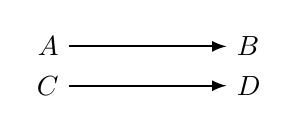
\begin{tikzpicture}
		\draw [thick,-latex] (0,1) node[anchor=east] {$A$} -- (2,1) node[anchor=west] {$B$};
		\draw [thick,-latex] (0,.5) node[anchor=east] {$C$} -- (2,.5) node[anchor=west] {$D$};
	\end{tikzpicture}
	\subsubsection{Opposite Vectors}
	Two vectors are opposite if they have the same magnitude but opposite direction. For example, $\vv{AB}=-\vv{CD}$ in the figure:\\
	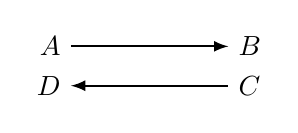
\begin{tikzpicture}
		\draw [thick,-latex] (0,1) node[anchor=east] {$A$} -- (2,1) node[anchor=west] {$B$};
		\draw [thick,latex-] (0,.5) node[anchor=east] {$D$} -- (2,.5) node[anchor=west] {$C$};
	\end{tikzpicture}\\
	As well, $\vv{AB}=-\vv{BA}$.
	\subsubsection{Parallel Vectors}
	Two vectors are parallel if their directions are either the same or opposite. If vectors $\vv{v_1}$ and $\vv{v_2}$ are parallel, you can write $\vv{v_1}\parallel\vv{v_2}$\\
	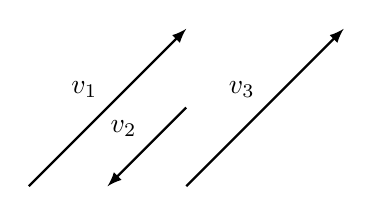
\begin{tikzpicture}
		\draw [thick, -latex] (0,0) -- (2,2) node [midway,above left]{$\vv{v_1}$};
		\draw [thick, latex-] (1,0) -- (2,1) node [midway,above left]{$\vv{v_2}$};
		\draw [thick, -latex] (2,0) -- (4,2) node [midway,above left]{$\vv{v_3}$};
	\end{tikzpicture}
	\subsubsection{Direction}
	To express the direction of a vector in a horizontal plane, we can either use:
	\begin{itemize}
		\item True (Azimuth) Bearing, the angle between North and the direction of the vector, measured clockwise. For example, 5m[120$^\circ$]
		\item Quadrant Bearing, the angle between North or South and the vector, towards East or West. For example, 5m[S60$^\circ$E]
	\end{itemize}
	\subsection{Vector Addition and Subtraction}
	\subsubsection{Addition of Two Vectors}
	The vector addition of two vectors $\vv{a}$ and $\vv{b}$ is denoted by $\vv{a}+\vv{b}$ and is called the sum or resultant of the two vectors
	\subsubsection{Triangle Rule (Tail to Tip Rule)}
	In order to find the sum of two geometric vectors, place the second vector with its tail on the tip of the first vector. The sum is the vector with its tail at the tail of the first vector and its head at the head of the second vector.
	%graph
	\subsubsection{Polygon Rule}
	To find the sum of $n$ geometric vectors, place each vector with its tail at the head of the previous vector.
	%graph
	\subsubsection{Parellogram Rule (Tail to Tail Rule)}
	To add two geometric vectors, you can also place their tails at the same point, and form a parellelogram using the vectors as the two sides. The sum is the diagonal of the parallelogram starting from the common tail point.
	%graph
	\subsubsection{Sine Law}
	For any triangle $\triangle ABC$, the following relation is true: $\dfrac{\sin A}{a}=\dfrac{\sin B}{b}=\dfrac{\sin C}{c}$
	%graph
	\subsubsection{Cosine Law}
	For any triangle $\triangle ABC$, the following relation is true and can be used with any combination of the sides and opposite angle: $c^2=a^2+b^2-2ab\cos C$
	%graph
	\subsubsection{Magnitude and Direction of Vector Sum}
	Let $\theta=\angle (\vv{a},\:\vv{b})$ be the angle between the vectors $\vv{a}$ and $\vv{b}$ when they are placed tail to tail. The magnitude of the vector sum is given by $\lVert\vv{a}+\vv{b}\rVert^2=\mv{a}^2+\mv{b}^2-2\mv{a}\mv{b}\cos(180^\circ-\theta)$. The direction of the vector sum $\vv{a}+\vv{b}$ is defined by the angles $\alpha$ and $\beta$ formed by the vector sum and the vectors $\vv{b}$ and $\vv{a}$ respectively: $\dfrac{\mv{a}}{\sin\alpha}=\dfrac{\mv{b}}{\sin\beta}=\dfrac{\lVert\vv{a}+\vv{b}\rVert}{\sin\gamma}$
	%diagram
	\subsubsection{Vector Subtraction}
	The subtraction operation between two vectors $\vv{a}-\vv{b}$ can be understood as the vector addition between the first vector and the opposite of the second vector: $\vv{d}=\vv{a}-\vv{b}=\vv{a}+\left(-\vv{b}\right)$
	%diagram
	\subsubsection{Inverse Operation}
	Vector subtraction is the inverse operator of vector addition: $\vv{d}=\vv{a}-\vv{b}\Leftrightarrow\vv{a}=\vv{b}+\vv{d}$
	\subsubsection{Magnitude and Direction of Vector Difference}
	If $\vv{d}=\vv{a}-\vv{b}$, and $\theta$ is the angle between $\vv{a}$ and $\vv{b}$ when they are placed tail to tail: %graph
	The magnitude of the vector difference is given by $\lVert\vv{a}-\vv{b}\rVert=\mv{a}^2+\mv{b}-2\mv{a}\mv{b}\cos\theta$
	\subsection{Multiplication of Vectors by Scalars}
	\subsubsection{Multiplication of a Vector by a Scalar}
	My multipying a vector $\vv{v}$ by a scalar $k$, we obtain a new vectot $k\vv{v}$ with the properties that $k\vv{v}$ has the same direction as $\vv{v}$ if $k>0$ and the opposite direction of $k<0$. As well, $\lVert k\vv{v}\rVert=|k|\times\mv{v}$
	\subsubsection{Properties}
	The following properties apply for the multiplication of a vector by a scalar:
	\begin{itemize}
		\item $k(\vv{a}+\vv{b})=k\vv{a}+k\vv{b}$
		\item $k(m\vv{a})=(km)\vv{a}=km\vv{a}$
		\item $(k+m)\vv{a}=k\vv{a}+m\vv{a}$
	\end{itemize}
	\subsubsection{Unit Vectors}
	A unit vector is a vector with a magnitude of 1. For any vector $\vv{v}$, a unit vector parallel to $\vv{v}$ is given by $\vv{u}=\dfrac{\vv{v}}{\mv{v}}$
	\subsection{Properties of Vectors}
	\subsubsection{Properties of Vectors}
	\begin{itemize}
		\item $\vv{a}+\vv{b}=\vv{b}+\vv{a}$
		\item $\vv{a}+0=0+\vv{a}=\vv{a}$
		\item $\vv{a}+(-\vv{a})=(-\vv{a})+\vv{a}=0$
		\item $(\vv{a}+\vv{b})+\vv{c}=\vv{a}+(\vv{b}+\vv{c})$
		\item $\lVert k\vv{a}\rVert=|k|\mv{a}$
		\item $k(\vv{a}+\vv{b})=k\vv{a}+k\vv{b}$
		\item $(kl)\vv{a}=k(l\vv{a})=l(k\vv{a})$
		\item $(k+l)\vv{a}=k\vv{a}+l\vv{a}$
		\item $1\vv{a}=\vv{a}$
		\item $-1(\vv{a})=-\vv{a}$
		\item $0\vv{a}=0$
		\item $\mv{0}=0$
	\end{itemize}
	\subsection{Vectors in $R^2$ and $R^3$}
	\subsubsection{Polar Coordinates}
	Given a Cartesian System of Coordinates, a 2D vector $\vv{v}$ may be defined by its magnitude $\mv{v}$ and the counter-clockwise angle $\theta$ between its positive direction of the x-axis and the vector.
	%graph
	The pair $(\lVert\vv{v}\rVert, \theta)$ determines the polar coordinates of the 2D vector and $\vv{v}=(\lVert\vv{v}\rVert, \theta)$.
	\subsubsection{Scalar Components for a 2D Vector}
	Let us consider a 2D vector with the tail in the origin of the Cartesian system. Parallels through its tip to the coordinate axes intersect the x-axis at $v_x$ and the y-axis at $v_y$.
	%graph
	The pair $(v_x, v_y)$ determines the scalar coordinates of the 2D vector and $\vv{v}=(v_x, v_y)$.
	\subsubsection{Link between Polar Coordinates and Scalar Components}
	To convert a vector from polar coordinates $\vv{v}=(\lVert\vv{v}\rVert,\:\theta)$ to scalar components $\vv{v}=(v_x,\:v_y)$, use the formulas $v_x=\lVert\vv{v}\rVert\cos\theta$ and $v_y=\lVert\vv{v}\rVert\sin\theta$\\
	To convert a vector from scalar components $\vv{v}=(v_x,\:v_y)$ to polar coordinates $\vv{v}=(\lVert\vv{v}\rVert,\:\theta)$, use the formulas $\lVert\vv{v}\rVert=\sqrt{{v_x}^2+{v_y}^2}$ and $\theta=\tan^{-1}\left(\dfrac{v_y}{v_x}\right)$
	\subsubsection{Magnitude of a 2D Algebraic Vector}
	The magnitude of a 2D algebraic vector $\vv{v}=(v_x,\:v_y)$ is given by $\lVert\vv{v}\rVert=\sqrt{{v_x}^2+{v_y}^2}$.
	\subsubsection{Standard Unit Vectors}
	The unit vectors $\vv{i}=(1,\:0)$ and $\vv{j}=(0,\:1)$ are called the standard unit vectors in 2D space.
	\subsubsection{Vector Components of a 2D Vector}
	Any vector $\vv{v}$ may be decomposed into two perpendicular vector components $\vv{v_x}$ and $\vv{v_y}$, parallel to each of the standard vectors. %graph
	The link between the scalar components and vector components is given by $\vv{v_x}=v_x\vv{i}$ and $\vv{v_y}=v_y\vv{j}$. A 2D vector may be written in algebraic form as $\vv{v}=\vv{v_x}+\vv{v_y}=v_x\vv{i}+v_y\vv{j}=\left(v_x,\:v_y\right)$
	\subsubsection{Position 2D Vector}
	The directed line segment $\vv{OP}$ from the origin $O$ to a generic point $P(x, y)$ determines a vector called a position vector, and $\vv{OP}=(x,\:y)=x\vv{i}+y\vv{j}$
	\subsubsection{Displacement 2D Vector}
	The directed line segment $\vv{AB}$ from the point $A(x_A, y_A)$ to the point $B(x_B, y_B)$ determines a vector called a displacment vector and $\vv{AB}=(x_B-x_A,\:y_B-y_A)=(x_B-x_A)\vv{i}+(y_B-y_A)\vv{j}$
	\subsubsection{Direction Angles}
	Let us consider a 3D coordinate system and a 3D vector $\vv{v}$ with a tail at the origin $O$. Direction angles are the angles $\alpha$, $\beta$, and $\gamma$ between the vector and the positive directions of the coordinate axes. %graph if 3D
	\subsubsection{Scalar Components of a 3D Vector}
	Let us consider a 3D coordinate system and a 3D vector $\vv{v}$ with a tail at the origin $O$. Parallel planes throught its tip to the coordinate planes intersec the x-axis at $v_x$, the y-axis at $v_y$, and the z-axis at $v_z$. The triple $(v_x,\:v_y,\:v_z)$ determines the scalar components of the 3D vector and $\vv{v}=(v_x,\:v_y,\:v_z)$. %graph
	\subsubsection{Link Between Direction Angles and 3D Scalar Components}
	The link between the direction angles ($\alpha$, $\beta$, and $\gamma$) and the scalar components ($v_x$, $v_x$, and $v_z$) is given by
	\begin{align*}
		v_x&=\mv{v}\cos\alpha&&&\alpha&=\cos^{-1}\left(\frac{v_x}{\mv{v}}\right)\\
		v_y&=\mv{v}\cos\beta&\text{and}&&\beta&=\cos^{-1}\left(\frac{v_y}{\mv{v}}\right)\\
		v_z&=\mv{v}\cos\gamma&&&\gamma&=\cos^{-1}\left(\frac{v_z}{\mv{v}}\right)\\
		&&\cos^2\alpha+\cos^2\beta&+\cos^2\gamma=1
	\end{align*}
	\subsubsection{Magnitude of a 3D Algebraic Vector}
	The magnitud of a vector $\vv{v}=(v_x,\:v_y,\:v_z)$ is given by $\mv{v}=\sqrt{{v_x}^2+{v_y}^2+{v_z}^2}$
	\subsubsection{3D Standard Unit Vectors}
	The unit vectors $\vv{i}=(1,\:0,\:0)$, $\vv{j}=(0,\:1,\:0)$, and $\vv{k}=(0,\:0,\:1)$ are called the standard unit vecors in 3D space. %graph
	\subsubsection{Vector components for a 3D Vector}
	Any 3D vector $\vv{v}$ may be decomposed into three perpendicular vector components
	\subsection{Operations with Vectors in $R^2$}
	\subsection{Operations with Algebraic Vectors in $R^3$}
	\tsection{Unit 7: Vector Applications}
	\setcounter{section}{7}
	\setcounter{subsection}{0}
	\subsection{Vectors as Forces}
	\subsection{Veolcity}
	\subsection{Dot Product of Two Geometric Vectors}
	\subsubsection{Definition}
	The dot product of two geometric vectors $\vv{a}$ and $\vv{b}$ with an angle $\angle(\vv{a},\:\vv{b})$ between them when placed tail to tail is a scalar defined by $\vv{a}\cdot\vv{b}=\mv{a}\mv{b}\cos\theta$. By convention, $0^\circ\leq\theta\leq180^\circ$. %graph
	\subsubsection{Properties of Dot Product}
	\begin{enumerate}
		\item $\vv{a}\cdot\vv{b}$ is a scalar (real number)
		\item If $\vv{a}\bot\vv{b}$, $\vv{a}\cdot\vv{b}=0$, because $\theta=90^\circ$, and $\cos90^\circ=0$
		\item If $\vv{a}\cdot\vv{b}=0$, then $\mv{a}=0$, $\mv{b}=0$, or $\vv{a}\bot\vv{b}$
		\item If $\ang{0}<\theta<\ang{90}$, then $\cos\theta>0$ and $\vv{a}\cdot\vv{b}>0$
		\item If $\ang{90}<\theta<\ang{180}$, then $\cos\theta<0$ and $\vv{a}\cdot\vv{b}<0$
		\item If $\vv{a}\uparrow\uparrow\vv{b}$, then $\theta=0$, $\cos\theta=1$, and $\vv{a}\cdot\vv{b}=\mv{a}\mv{b}$
	\end{enumerate}
	\subsection{Dot Product of Algebraic Vectors}
	\subsubsection{Dot Product of Standard Unit Vectors}
	The dot product of any two of the same standard unit vectors is equal to 1, and he dot productt of any two different standard unit vectors is 0, because
	\[\vv{i}\cdot\vv{i}=\mv{i}\mv{i}\cos\ang{0}=(1)(1)(1)=1\]\[\vv{i}\cdot\vv{j}=\mv{i}\mv{j}\cos\ang{90}=(1)(1)(0)=0 \text{ (they are perpendicular).}\]
	\subsubsection{Dot Product of Two Algebraic Vectors}
	The dot product of two algebraic vectors $\vv{a}=(a_x,\:a_y,\:a_z)=a_x\vv{i}+a_y\vv{j}+a_z\vv{k}$ and $\vv{b}=(a_x,\:a_y,\:a_z)=a_x\vv{i}+a_y\vv{j}+a_z\vv{k}$ is given by
	\subsection{Scalar Projection and Vector Projection}
	\subsubsection{Scalar Projection}
	The scalar projection of the vector $\vv{a}$ onto vector $\vv{b}$ is a scalar defined as $\mv{a}\cos\theta$, where $\theta=\angle(\vv{a},\:\vv{b})$
	\subsubsection{Special Cases}
	\begin{itemize}
		\item If $\vv{a}\uparrow\uparrow\vv{b}$, $\cos\theta=1$, and $s=\mv{a}$
		\item If $\vv{a}\uparrow\downarrow\vv{b}$, $\cos\theta=-1$, and $s=-\mv{a}$
		\item If $\vv{a}\bot\vv{b}$, $\cos\theta=0$, and $s=0$
	\end{itemize}
	\subsubsection{Dot Product and Scalar Projection}
	Since the dot product is defined as $\vv{a}\cdot\vv{b}=\mv{a}\mv{b}\cos\theta$, the scalar projection can be rewritten as $s=\mv{a}\cos\theta=\dfrac{\vv{a}\cdot\vv{b}}{\mv{b}}$
	\subsection{Cross Product of Two Vectors}
	\subsubsection{Right Hand System}
	The Right Hand System is based on the position of the first three fingers of the right hand: %illustrated
	\subsubsection{Corkscrew Rule}
	The corkscrew rule describes a right hand system based on the corkscrew property: if you rotate the x-axis towards the y-axis using the shortest path, the screw goes in the positive direction of the z-axis
	\subsubsection{Cross Product}
	The cross product between two vectors $\vv{a}$ and $\vv{b}$ is a vector quantity denoted by $\vv{a}\times\vv{b}$ having the following properties
	\begin{itemize}
		\item $\lVert\vv{a}\times\vv{b}\rVert=\mv{a}\mv{b}\sin\theta$
		\item $\vv{a}\times\vv{b}$ is perpendicular to both $\vv{a}$ and $\vv{b}$ (is perpendicular to the plane determined by $\vv{a}$ and $\vv{b}$
		\item The vectors $\vv{a}$, $\vv{b}$, and $\vv{a}\times\vv{b}$ form a right-handed system
	\end{itemize}
	\subsubsection{Specific Cases}
	\begin{itemize}
		\item If $\vv{a}\parallel\vv{b}$ ($\theta=0$ or $\theta=\pi=\ang{180})$, then $\vv{a}\times\vv{b}=0$
		\item If $\vv{a}\bot\vv{b}$ $\left(\theta=\dfrac{\pi}{2}=\ang{90}\right)$, then $\lVert\vv{a}\times\vv{b}\rVert=\mv{a}\mv{b}$ (the maximum)
		\item If $\vv{a}=\vv{b}$, then $\vv{a}\times\vv{b}=0$
	\end{itemize}
	
	
	
	\section{Have to Figure Out Where This Goes}
	\[y=\frac{x|x|}{x+3}=\begin{cases}
		-\frac{x^2}{x+3}&x<0\\
		\frac{x^2}{x+3}&x\geq0
	\end{cases}\]
	\[\text{Domain: }\{x\in\mathbb{R}\mid x\neq-3\}\]
	\[\text{Vertical Asymptote at }x=-3\text{ as }\]
	% as x -> -3- y->inf
	% as x -> -3+ y->-inf
	%zero at 0,0
	%divisions statement, as x-> -inf =-x+3
	%as x-> inf y=x-3
	
	%- from the left
	%+ from the right
	%zeroes of the numerator that are not numerators are x intercepts
	%rational function is p/q, q!=0
	%holes are common factors
	%vertical asymptotes are unique roots of q(x)
	%no holes or vertical asymptotes when domain is all real x
	%you can determine the behavior around the vertical asymptotes
	%x-intercepts are unique roots of p(x)
	%y-intercepts if 0 is part of the domain
	%end behavior comes from when |x| approaches infinity (lim f(x) |x|\to\infty)=a_nx^n/b_mx^m
	%y=(x|x|)/(x-3) splits because of the absolute value, vertical asymptote
	
	%graph with no value at x=a
	\noindent Left hand limit (the value when it is approaching from the left):\[L=\lim_{x\to a^-}f(x)\]
	Right hand limit (the value when it is approaching from the right):\[R=\lim_{x\to a^+}f(x)\]
	Lowercase l limit : 
	%lowercase l can be either equal to L or R when L = R
	%hole or removable disconinuity, L = 1, R = 1, 
	%even if f(1)=3/2, lowercase l = 1
	%0/0 is indeterminate case, if you plug it into the equation, also inf/inf, inf-inf, 1^inf, 0^0, inf^0
	
	%n^2+1/n
\end{document}
